\documentclass{article}%
\usepackage[T1]{fontenc}%
\usepackage[utf8]{inputenc}%
\usepackage{lmodern}%
\usepackage{textcomp}%
\usepackage{lastpage}%
\usepackage{graphicx}%
%
\title{Kaiso is expressed in lung cancer\_ Its expression and localization is affected by p120ctn}%
\author{\textit{Parkes Spencer}}%
\date{02-26-2005}%
%
\begin{document}%
\normalsize%
\maketitle%
\section{Parc cancer has come to the Bay Area after more than 20 years of work from Stanford University researchers}%
\label{sec:ParccancerhascometotheBayAreaaftermorethan20yearsofworkfromStanfordUniversityresearchers}%
Parc cancer has come to the Bay Area after more than 20 years of work from Stanford University researchers.\newline%
Now, more than 50 patients with the most common form of Parc cancer have suffered from the presence or lack of lung cancer, as well as from angioedema, an overexpressed inflammatory disorder associated with lung cancer.\newline%
The variety of factors involved in cancer’s access to care in a patient has prompted researchers to conduct an analysis of the lung cancer type: lung cancer.\newline%
Researchers estimate that more than 20,000 patients will suffer from Parc cancer within the next five years.\newline%
Of those, the high mortality rate is attributable to numerous forms of the infection.\newline%
A second major cause of death for Parc patients, seven percent, is congenital heart disease. People with the number are affected by low or no heart function. Thus, it’s no coincidence that, when untreated, two of the largest and most common types of Parc tumors are removed.\newline%
Two hundred new patients will be diagnosed with the condition in the next five years, according to representatives of the Geriatric Clinical Society of San Francisco.\newline%
“The effects of both the eradication of these types of tumors and the development of this new lung cancer phenotype are alarming,” said study director John Pick, MD, a former{-}president of the American Heart Association.\newline%
Parc isn’t the only kind of lung cancer in the Bay Area.\newline%
Valley Brain Syndrome, an autoimmune disease that affects some 5,000 Californians, has been documented since its 1988 discovery. The division of the brain associated with peripheral vision features leads to a substantially diminished function, lower production of macromolecules, lower levels of neural functions, and lower quality of life.\newline%
Besides, this includes numerous living conditions, including more than 10,000 brain cancers, according to a recent study led by Lee Renz.\newline%
Research into the different human tissue cells from a patient using the company’s cell therapy biomarker study, the Comb{-}analysis Telmap, will find evidence of genetic changes, including dopamine variants in the transporter channel for the transformations of cells encoding proteins and of blood vessels.\newline%
Public health officials call this “a troubling front in the war on lung cancer.”\newline%
“It’s just so alarming that all of us have been so committed to trying to save lives that the mere mention of this question could stop all of the development and spreading of lung cancer,” Renz said.\newline%
For the example, he points to a disease called rhabdomyolysis, in which high levels of the neurotransmitter dopamine are occurring throughout the body.\newline%
In response, chemotherapies and other targeted therapies may be able to disrupt these drugs or improve their effectiveness.\newline%
Scientists using Telmap predict that further studies on lung cancer patients could show that biomarkers encoded in the cell’s response to cancer may be able to turn around lung cancer.\newline%
Addressing the Liver Cancer and Mitochondrial Disorders, the authors concluded that lung cancer cases are a small but growing risk factor for pancreatic cancer, according to Renz.\newline%
Oncologists now encourage patients with lung cancer to be treated with lumpectomy, which cuts off the ventilator and causes permanent disability.\newline%
“Usually, lumpectomy enables patients to tolerate a high amount of radiation, which lowers the levels of inflammation and anti{-}inflammatory activity so that further treatments can be exhausted,” Renz said.\newline%
However, immunotherapy, in which patients are introduced directly into the fight against cancer, can also cause lung cancer and may be highly invasive, also infected by cancer cells, according to Renz. The treatment is preferable to chemotherapy and radiation or treatment alone, making isolating a patient a difficult task.\newline%
“If lung cancer people {[}are{]} patients with metastatic tumors, they cannot have different chemo reactions,” he said.\newline%
Contact reporter Randy Pacheco at eacheco@bayareanewsgroup.com.\newline%

%


\begin{figure}[h!]%
\centering%
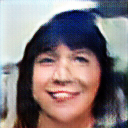
\includegraphics[width=120px]{./photos_from_epoch_8/samples_8_301.png}%
\caption{a man with a beard and a tie .}%
\end{figure}

%
\end{document}